\section{Introduction to tools}
These are the tools that help us to reduce the work of the developer by just providing the function ready for the direct usage.

\subsection{OSMnx}

\begin{figure}[h]
\centering 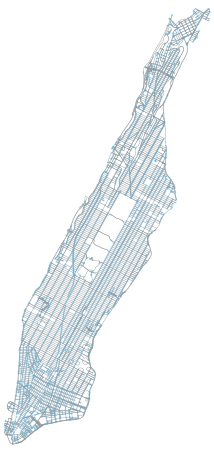
\includegraphics[scale=0.50]{input/images/osmnx.png}
\caption{OSMnx map of manhattan}
\end{figure}
OSMnx: retrieve, construct, analyze, and visualize street networks from OpenStreetMap. OSMnx is a Python package that lets you download spatial geometries and construct, project, visualize, and analyze street networks from OpenStreetMap’s APIs. Users can download and construct walkable, drivable, or bikable urban networks with a single line of Python code, and then easily analyze and visualize them.\\

{\bf Features}
\begin{itemize}
\item Download street networks anywhere in the world with a single line of code
\item Download other infrastructure network types, place polygons, or building footprints as well
\item Download by city name, polygon, bounding box, or point/address + network distance
\item Get drivable, walkable, bikable, or all street networks
\item Visualize the street network as a static image or leaflet web map
\item Simplify and correct the network’s topology to clean and consolidate intersections
\item Save networks to disk as shapefiles or GraphML
\item Conduct topological and spatial analyses to automatically calculate dozens of indicators
\item Calculate and plot shortest-path routes as a static image or leaflet web map
\item Plot figure-ground diagrams of street networks and/or building footprints
\item Download node elevations and calculate edge grades
\item Visualize travel distance and travel time with isoline and isochrone maps
\item Calculate and visualize street bearings and orientations\\

\end{itemize}


{\bf Installation}
\begin{verbatim}
$ sudo apt-get install python-pip python-virtualenv
$ virtualenv venv
$ source venv/bin/activate
$ pip install osmnx
\end{verbatim}

{\bf Usage}
\begin{verbatim}
import osmnx as ox
G = ox.graph_from_place('Punjab, India', network_type='drive')
ox.plot_graph(ox.project_graph(G))
\end{verbatim}


\subsection{NetworkX}

\begin{figure}[h]
\centering 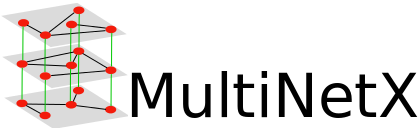
\includegraphics[scale=0.5]{input/images/networkx.png}
\caption{NetworkX logo}
\end{figure}

NetworkX is a Python package for the creation, manipulation, and study of the structure, dynamics, and functions of complex networks.\\

  
{\bf Features}
\begin{itemize}
    \item Data structures for graphs, digraphs, and multigraphs
    \item Many standard graph algorithms
    \item Network structure and analysis measures
    \item Generators for classic graphs, random graphs, and synthetic networks
    \item Nodes can be "anything" (e.g., text, images, XML records)
    \item Edges can hold arbitrary data (e.g., weights, time-series)
    \item Open source 3-clause BSD license
    \item Well tested with over 90\% code coverage
    \item Additional benefits from Python include fast prototyping, easy to teach, and multi-platform
\end{itemize}

{\bf Installation}
\begin{verbatim}
$ sudo apt-get install python-pip python-virtualenv
$ virtualenv venv
$ source venv/bin/activate
$ pip install networkx
\end{verbatim}

{\bf Algorithm}
PageRank computes a ranking of the nodes in the graph G based on the structure of the incoming links. It was originally designed as an algorithm to rank web pages.\\


{\bf Graph types}
\begin{itemize}
\item Undirected Simple
\item Directed Simple
\item With Self-loops
\item With Parallel edges

\end{itemize}


\subsection{GraphFrames}

\\GraphFrames is a package for Apache Spark which provides DataFrame-based Graphs. It provides high-level APIs in Scala, Java, and Python. It aims to provide both the functionality of GraphX and extended functionality taking advantage of Spark DataFrames. This extended functionality includes motif finding, DataFrame-based serialization, and highly expressive graph queries.\\

{\bf What are GraphFrames?}\\
GraphX is to RDDs as GraphFrames are to DataFrames.\\

GraphFrames represent graphs: vertices (e.g., users) and edges (e.g., relationships between users). If you are familiar with GraphX, then GraphFrames will be easy to learn. The key difference is that GraphFrames are based upon Spark DataFrames, rather than RDDs.\\

GraphFrames also provide powerful tools for running queries and standard graph algorithms. With GraphFrames, you can easily search for patterns within graphs, find important vertices, and more. Refer to the User Guide for a full list of queries and algorithms.\\


{\bf creating nodes using pagerank algorithm}
\begin{verbatim}
# Create a Vertex DataFrame with unique ID column "id"
v = sqlContext.createDataFrame([
  ("a", "Alice", 34),
  ("b", "Bob", 36),
  ("c", "Charlie", 30),
], ["id", "name", "age"])

# Create an Edge DataFrame with "src" and "dst" columns
e = sqlContext.createDataFrame([
  ("a", "b", "friend"),
  ("b", "c", "follow"),
  ("c", "b", "follow"),
], ["src", "dst", "relationship"])

# Create a GraphFrame
from graphframes import *
g = GraphFrame(v, e)

# Query: Get in-degree of each vertex.
g.inDegrees.show()

# Query: Count the number of "follow" connections in the graph.
g.edges.filter("relationship = 'follow'").count()

# Run PageRank algorithm, and show results.
results = g.pageRank(resetProbability=0.01, maxIter=20)
results.vertices.select("id", "pagerank").show()
\end{verbatim}

\subsection{Django}
\begin{figure}[h]
	\centering 
\includegraphics[scale=0.2]{input/images/django.png}
	\caption{Django logo}
\end{figure}
\subsubsection{What is Django?}
Django is a high-level Python web framework that enables rapid development of secure and maintainable websites. Built by experienced developers, Django takes care of much of the hassle of web development, so you can focus on writing your app without needing to reinvent the wheel. It is free and open source, has a thriving and active community, great documentation, and many options for free and paid-for support. \\

Django helps you write software that is:
\\
Django follows the "Batteries included" philosophy and provides almost everything developers might want to do "out of the box". Because everything you need is part of the one "product", it all works seamlessly together, follows consistent design principles, and has extensive and up-to-date documentation.\\
Django can be (and has been) used to build almost any type of website — from content management systems and wikis, through to social networks and news sites. It can work with any client-side framework, and can deliver content in almost any format (including HTML, RSS feeds, JSON, XML, etc). The site you are currently reading is based on Django!\\
Django helps developers avoid many common security mistakes by providing a framework that has been engineered to "do the right things" to protect the website automatically. For example, Django provides a secure way to manage user accounts and passwords, avoiding common mistakes like putting session information in cookies where it is vulnerable (instead cookies just contain a key, and the actual data is stored in the database) or directly storing passwords rather than a password hash.\\

A password hash is a fixed-length value created by sending the password through a cryptographic hash function. Django can check if an entered password is correct by running it through the hash function and comparing the output to the stored hash value. However due to the "one-way" nature of the function, even if a stored hash value is compromised it is hard for an attacker to work out the original password.\\

Django enables protection against many vulnerabilities by default, including SQL injection, cross-site scripting, cross-site request forgery and clickjacking (see Website security for more details of such attacks).\\

Django uses a component-based “shared-nothing” architecture (each part of the architecture is independent of the others, and can hence be replaced or changed if needed). Having a clear separation between the different parts means that it can scale for increased traffic by adding hardware at any level: caching servers, database servers, or application servers. Some of the busiest sites have successfully scaled Django to meet their demands (e.g. Instagram and Disqus, to name just two).\\
Django code is written using design principles and patterns that encourage the creation of maintainable and reusable code. In particular, it makes use of the Don't Repeat Yourself (DRY) principle so there is no unnecessary duplication, reducing the amount of code. Django also promotes the grouping of related functionality into reusable "applications" and, at a lower level, groups related code into modules (along the lines of the Model View Controller (MVC) pattern).\\
\subsubsection{Where did it come from?}
Django was initially developed between 2003 and 2005 by a web team who were responsible for creating and maintaining newspaper websites. After creating a number of sites, the team began to factor out and reuse lot of common code and design patterns. This common code evolved into a generic web development framework, which was open-sourced as the "Django" project in July 2005. \\

Django has continued to grow and improve, from its first milestone release (1.0) in September 2008 through to the recently-released version 1.11 (2017). Each release has added new functionality and bug fixes, ranging from support for new types of databases, template engines, and caching, through to the addition of "generic" view functions and classes (which reduce the amount of code that developers have to write for a number of programming tasks). \\
\subsubsection{How popular is Django?}
There isn't any readily-available and definitive measurement of popularity of server-side frameworks (although sites like Hot Frameworks attempt to assess popularity using mechanisms like counting the number of GitHub projects and StackOverflow questions for each platform). A better question is whether Django is "popular enough" to avoid the problems of unpopular platforms. Is it continuing to evolve? Can you get help if you need it? Is there an opportunity for you to get paid work if you learn Django?\\ 

Based on the number of high profile sites that use Django, the number of people contributing to the codebase, and the number of people providing both free and paid for support, then yes, Django is a popular framework!\\

High-profile sites that use Django include: Disqus, Instagram, Knight Foundation, MacArthur Foundation, Mozilla, National Geographic, Open Knowledge Foundation, Pinterest, and Open Stack\\

\subsubsection{Is Django opinionated?}
Web frameworks often refer to themselves as "opinionated" or "unopinionated".\\

Opinionated frameworks are those with opinions about the "right way" to handle any particular task. They often support rapid development in a particular domain (solving problems of a particular type) because the right way to do anything is usually well-understood and well-documented. However they can be less flexible at solving problems outside their main domain, and tend to offer fewer choices for what components and approaches they can use.\\

Unopinionated frameworks, by contrast, have far fewer restrictions on the best way to glue components together to achieve a goal, or even what components should be used. They make it easier for developers to use the most suitable tools to complete a particular task, albeit at the cost that you need to find those components yourself.\\

Django is "somewhat opinionated", and hence delivers the "best of both worlds". It provides a set of components to handle most web development tasks and one (or two) preferred ways to use them. However, Django's decoupled architecture means that you can usually pick and choose from a number of different options, or add support for completely new ones if desired.\\
\subsubsection{What does Django code looks like?}
In a traditional data-driven website, a web application waits for HTTP requests from the web browser (or other client). When a request is received the application works out what is needed based on the URL and possibly information in POST data or GET data. Depending on what is required it may then read or write information from a database or perform other tasks required to satisfy the request. The application will then return a response to the web browser, often dynamically creating an HTML page for the browser to display by inserting the retrieved data into placeholders in an HTML template.\\

Django web applications typically group the code that handles each of these steps into separate files:\\
\begin{figure}[h]
	\centering 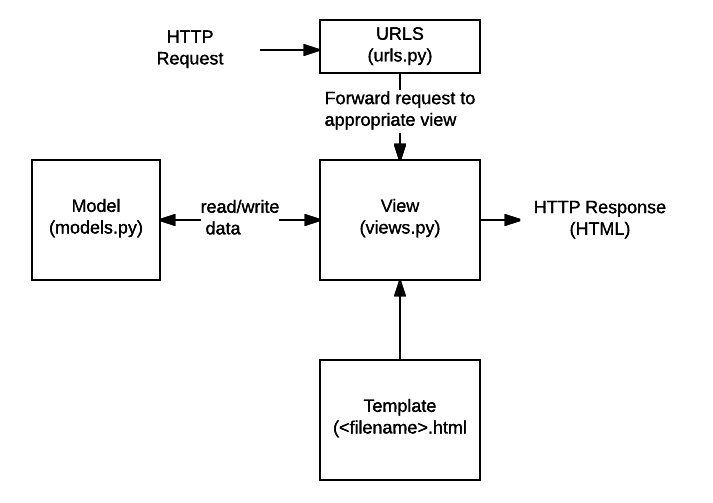
\includegraphics[scale=1]{input/images/django1.png}
	\caption{Django logo}
\end{figure}
\begin{itemize}
	\item URLs: While it is possible to process requests from every single URL via a single function, it is much more maintainable to write a separate view function to handle each resource. A URL mapper is used to redirect HTTP requests to the appropriate view based on the request URL. The URL mapper can also match particular patterns of strings or digits that appear in an URL, and pass these to a view function as data.
	\item View: A view is a request handler function, which receives HTTP requests and returns HTTP responses. Views access the data needed to satisfy requests via models, and delegate the formatting of the response to templates.
	\item Models: Models are Python objects that define the structure of an application's data, and provide mechanisms to manage (add, modify, delete) and query records in the database. 
	\item Templates: A template is a text file defining the structure or layout of a file (such as an HTML page), with placeholders used to represent actual content. A view can dynamically create an HTML page using an HTML template, populating it with data from a model. A template can be used to define the structure of any type of file; it doesn't have to be HTML!
\end{itemize}

\subsection{Apache Spark}
\begin{figure}[h]
	\centering 
\includegraphics[scale=0.2]{input/images/spark.png}
	\caption{Apache Spark logo}
\end{figure}
We are aware that today we have huge data being generated everywhere from various sources. This data is either being stored intentionally in a structured way or getting generated by machines. But data is of no use until we mine it and try to do some kind of analysis on it, in order to come up with actions based on the analysis outcomes. The act of gathering and storing information for eventual analysis is ages old but it had never been based on such a large amount of data, which is there today. There is a specific term for such voluminous data i.e. “Big Data”.

Big data is a term that describes the huge volume of data which can be structured and unstructured or semi-structured. But it’s not the amount of data which is a concern for the organizations since it is just a storage problem which can be easily addressed by the cheap storage available today. It’s what Business get out of the data matters.Big data can be analyzed for insights that lead to better decisions and strategic business moves.

This problem can be solved if we have a framework which not only gives a solution to store all kinds of data (structured, semi-structured or unstructured) but an efficient way of analyzing it according to business needs. One of such framework which is widely used is known as Hadoop. But Hadoop has several limitation (which will be discussed in later sections), because of which Apache Spark was created.

Now we have a solution for our storage and also an efficient way of analyzing data of any size. That means we can make business decisions after analyzing data. But there is another challenge, which is that the decision based on the analysis insight on a huge data might not be relevant after some time. Any decision is useful if we take the action on time, but doing any analysis on huge data takes time, sometimes more than the deadline on which that action had to be performed. So in such cases such insights are of no use because the deadline for action has passed.Processing larger scale of data with Hadoop’s processing framework i.e. MapReduce (MR) is far better than our traditional system but still not good enough for organizations to take all its decision on time, because Hadoop operates on batch processing of data leading to high latency.

Several other shortcomings of Hadoop are:\\

\begin{itemize}
	\item Adherence to its MapReduce programming model
	\item Limited programming language API options
	\item Not a good fit for iterative algorithms like Machine Learning Algorithms
	\item Pipelining of tasks is not easy
\end{itemize}
\subsubsection{What is Spark?}
Apache Spark is an open source data processing framework for performing Big data analytics on distributed computing cluster.

Spark was initially started by Matei Zaharia at UC Berkeley's AMPLab in 2009. It was an academic project in UC Berkley. Initially the idea was to build a cluster management tool, which can support different kind of cluster computing systems. The cluster management tool which was built as a result is Mesos. After Mesos was created, developers built a cluster computing framework on top of it, resulting in the creating of Spark.

Spark was meant to target interactive iterative computations like machine learning. In the year 2013, the spark project was passed on to the Apache Software Foundation.

Spark has several advantages when compared to other big data and MapReduce technologies like Hadoop and Storm. Spark is faster than MaReduce and offers low latency due to reduced disk input and output operation. Spark has the capability of in memory computation and operations, which makes the data processing really fast than other MapReduce.

Unlike Hadoop spark maintains the intermediate results in memory rather than writing every intermediate output to disk. This hugely cuts down the execution time of the operation, resulting in faster execution of task, as more as 100X time a standard MapReduce job. Apache Spark can also hold data onto the disk. When data crosses the threshold of the memory storage it is spilled to the disk. This way spark acts as an extension of MapReduce. Spark doesn’t execute the tasks immediately but maintains a chain of operations as meta-data of the job called DAG. The action on the DAG happens only when an action operation is called on to the transformation DAG. This process is called as lazy evaluation. This allows optimized execution of the queries on Big Data.

Apache Spark has other features, such as:
\\
\begin{itemize}
	\item Supports wide variety of operations, compared to Map and Reduce functions.
	\item Provides concise and consistent APIs in Scala, Java and Python.
	\item Spark is written in Scala Programming Language and runs in JVM.
	\item It currently has support in  the following programming languages to develop applications in Spark:
	\subitem Scala
	\subitem Java
	\subitem Python
	\subitem R
	\item Features interactive shell for Scala and Python. This is not available in Java yet.
	\item It leverages the distributed cluster memory for doing computations for increased speed and data processing.
	Spark enables applications in Hadoop clusters to run up to as much as 100 times faster in memory and 10 times faster even when running in disk.
	It is most suitable for real time decision making with big data.
	\item It runs on top of existing Hadoop cluster and access Hadoop data store (HDFS), it can also process data stored by HBase structure. It can also run without Hadoop with apache Mesos or alone in standalone mode.
	\item Apache Spark can be integrated with various data sources like SQL, NoSQL, S3, HDFS, local file system etc.
	Good fit for iterative tasks like Machine Learning (ML) algorithms.
	\item In addition to Map and Reduce operations, it supports SQL like queries, streaming data, machine learning and data processing in terms of graph.
\end{itemize}
\subsubsection{Hadoop and Spark}
Hadoop as a big data processing technology has proven to be the go to solution for processing large data sets. MapReduce is a great solution for computations, which needs one-pass to complete, but not very efficient for use cases that require multi-pass for computations and algorithms. Each stage in the data processing workflow has one Map and one Reduce phase .To leverage MapReduce solution we need to convert our use case into MapReduce pattern. The Job's output data between each step has to be stored in the file system before the next step can begin. Hence, this approach is slow, due to replication \& disk Input/output operations. Also, Hadoop ecosystem doesn’t have every component to complete a big data use case. It also requires the integration of several other tools for different big data use cases (like Mahout for Machine Learning and Storm for streaming data processing, Flume for log aggregation).

If you want to do an iterative job, you would have to stitch together a sequence of MapReduce jobs and execute them in sequence. Each of those jobs has high-latency, and each depends upon the completion of previous stages. Spark allows programmers to employ complex, multi-step data pipelines using directed acyclic graph (DAG) pattern. It allows in-memory data sharing across DAGs, so that different jobs can work with the same data without going to disk.

Spark can run on top of Hadoop’s distributed file system Hadoop Distributed File System (HDFS) to leverage the distributed replicated storage. Spark can be used along with MapReduce in the same Hadoop cluster or can be used alone as a processing framework. Apache Spark is an alternative to Hadoop MapReduce rather than a replacement of Hadoop. It’s not intended to replace Hadoop but it can regarded as an extension to it. In many use cases MapReduce and Spark can be used together where MapReduce job can be used for batch processing and spark can be used for real-time processing.

\subsubsection{Apache Spark and its components}

SparkContext is an independent process through which spark application runs over a cluster. It gives the handle to the distributed mechanism/cluster so that you may use the resources of the distributed machines in your job. Your application program which will use SparkContext object would be known as driver program. Specifically, to run on a cluster, the SparkContext connects to several types of cluster managers (like Spark’s own standalone cluster manager, apache Mesos or Hadoop's YARN), which allocate resources across applications. Once connected, Spark takes over executors on distributed nodes in the cluster, which are processes in the distributed nodes that run computations and store data for your application. Next, it sends your application code to the executors through SparkContext. Finally tasks are sent to the executors to run and complete it.
\\
\begin{figure}[h]
	\centering 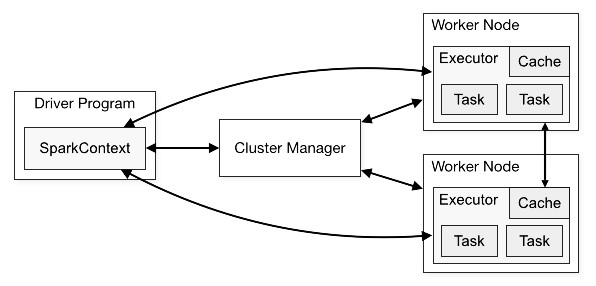
\includegraphics[scale=1]{input/images/spark1.jpg}
	\caption{Spark cluster overview}
	
\end{figure}

\subsubsection{Spark SQL, DataFrames and Datasets}
\begin{itemize} 
\item \textbf{SQL:}
Spark SQL exposes spark APIs to run SQL query like computation on large data. A spark user can perform ad-hoc query and perform near real time ETL on a different types of data like (like JSON, Parquet, Database).

\item \textbf{DataFrames:}
A DataFrame can be considered as a distributed set of data which has been organized into many named columns. It can be compared with a relational table, CSV file or a data frame in R or Python. The DataFrame functionality is made available as API in Scala, Java, Python, and R.

\item \textbf{Dataset:}
A Dataset is a new addition in the list of spark libraries. It is an experimental interface added in Spark 1.6 that tries to provide the benefits of RDDs with the benefits of Spark SQL’s optimized execution engine.

\item \textbf{Spark MLlib And ML:}
MLlib is collective bunch few handy and useful machine learning algorithms and data cleaning and processing approaches which includes classification, clustering, regression, feature extraction, dimensionality reduction, etc. as well as underlying optimization primitives like SGD and BFGS.

\item \textbf{Spark GraphX:}
GraphX is the Spark API for graphs and graph-parallel computation. GraphX enhances the Spark RDD by introducing the Resilient Distributed Property Graph.

A RDD property graph is a directed multi-graph with properties attached with each of its vertex and edge. GraphX has a set of basic operators (like subgraph, joinVertices, aggregateMessages, etc.).Along with operators it has an optimized variant of the Pregel API. GraphX is still under development and many developers are working towards simplification of graph related tasks.

\end{itemize}
